% The entire content of this work (including the source code
% for TeX files and the generated PDF documents) by 
% Hongxiang Chen (nicknamed we.taper, or just Taper) is
% licensed under a 
% Creative Commons Attribution-NonCommercial-ShareAlike 4.0 
% International License (Link to the complete license text:
% http://creativecommons.org/licenses/by-nc-sa/4.0/).
\documentclass{article}

% My own physics package
% The following line load the package xparse with additional option to
% prevent the annoying warnings, which are caused by the package
% "physics" loaded in package "physicist-taper".
\usepackage[log-declarations=false]{xparse}
\usepackage{physicist-taper}

\makenomenclature

\title{Notes for Classification of topological quantum matter with
symmetries}
\date{\today}
\author{Taper}


\begin{document}


\maketitle
\abstract{
As title suggests.
}
\tableofcontents
\section{Doubts}
\label{sec:Doubts}

\paragraph{Asks}
\begin{enumerate}
    \item Page 6. Why the scalar in Schur's lemma becomes of unit lenght.
    \item page 9. What does it mean by:
        \begin{quote}
            Note that unitary symmetries, which commute with the
            Hamiltonian, allow us to bring the Hamiltonian into a
            block diagonal form.
        \end{quote}
    \item page 9, table I. When he talks about \textit{codimension},
        what is the dimension of the whole space? ($3$? $3+1$?).
        Similar problem also exists in page 10.
        Note, he mentions codimension of gaples modes on page 11. He
        asserts that codimension $1$ means $1$ dimension less than the
        bulk. But it should be strange to compare the dimension of
        defects with the dimension of the bulk.

        Possibly related
        resources:\href{http://www.virginia.edu/bohr/mse209/chapter4.htm}
        {Online notes about Imperfection}:
        \begin{itemize}
            \item $0$D (zero dimension) – point defects: vacancies and
                interstitials. Impurities.
            \item 1D – linear defects: dislocations (edge, screw,
                mixed) 
            \item 2D – grain boundaries, surfaces.  
            \item 3D – extended defects: pores, cracks.
        \end{itemize}

        Note: it is finally defined on page 12. that is:
        codimension of defect $d_c:= d_\text{bulk} - d_\text{defect}$.
    \item page 6, what does it mean by saying \textit{"unitary
        symmetry"}.
    \item page 10, what is a \textit{"quantum phase diagram"}.
    \item page 11, what does he says, \textit{"Topological properties of
        adiabatic cycles can also be discussed in a similar manner."}.
        Does this mean that all previous classification does not
        concern the adiabatic cycles? What is \textit{"adiabatic
        cycles"} exactly in his language?

        Note: "adiabatic cycle" may refer to a cycle in phase space
        (most likely argumented by time $t$ parameter). "Adiabatic"
        describes the process to be adiabatical, i.e. vary very
        slowly. The detailed criterion is on page 12, just above
        equation 3.6:
        \begin{equation}
            \xi \abs{\Delta_r H(k,r)}<<\varepsilon_g
        \end{equation}
    \item page 12, "disinclination" is what kind of defect? Any books
        on crystall defects?
    \item page 12, is the \textit{"mass gap"} a massive gap or a gap
        composed of mass?
    \item page 12, about the $D$: if $d_c=1$ (line defect in a
        $2d$-bulk), then $D=0$. So a line is wrapped by a point?
        also, on fig. 2, the ($D=2,d=1$) gives a $d_\text{defect}=-1$!
        Judging from this graph, a $d_\text{defect}=-1$ means a
        temporal defect. Is this true?
    \item page 42, what is a nodal system, what are nodal points?
\end{enumerate}

\paragraph{Ask friends}
\begin{enumerate}
    \item page 13. What is a homotopy type?
\end{enumerate}
\paragraph{Doubts}
\begin{enumerate}
    \item page 10. Amazingly, he says, \textit{"all TIs and TSCs in
        the ten AZ symmetry classes are stable against disorder, and
        hence the assumption of translation invariance is not at all
        necessary"}.  How can translational invariance be ignored?
    \item page 12, he mentions:
        \begin{quote}
            As in the case of gapped TIs and TSCs, we are interested
            in the highest dimension strong topologies of the defect
            that do not involve lower dimensional cycles
        \end{quote}
        I don't get what "strong topologies" and "lower dimensional
        cycles" mean.
    \item page 13 right column, again he mentioned the strong topology
        and compactify the space into a $S^{d+D}$. I don't get why:
        \begin{quote}
            Physically this means the defect band theory are assumed
            to have trivial winding around those low-dimensional
            cycles.
        \end{quote}
        
    \item page 13, What does this mean:
        \begin{quote}
            It deformation retracts from the defect complement of
            spacetime.
        \end{quote}
        
\end{enumerate}

\paragraph{Revisit}
\begin{enumerate}
    \item page 12, bottom. How this procedure of relating real and
        complex classification is done?
\end{enumerate}
\section{Summary}
\label{sec:Summary}

\subsection{About topological matter}
\label{sec:About-topological-matter}
Topological states:
\begin{itemize}
    \item Topological insulators cannot be distinguished from
        ordinary, topologically trivial insulators in terms of their
        symmetries.
    \item topological insulators' topological nontriviality cannot be
        detected by a local order parameter.
    \item insulating electronic band structures can be categorized in
        terms of topology.
    \begin{itemize}
        \item time-reversal are crucial in makeing a spin-orbit induced
            topological insulators. $ \Rightarrow$ symmetry-protected
            topological phases (\nomen{SPT}).
        \item symmetry-protected topological phase can also arise from
            spatial symmetry.
    \end{itemize}
    \item There is a direct analogy between \nomen{TI}s and
        \nomen{TSC}s (topological insulators and topological
        superconductors).
    \item \nomen{bulk-boundary correspondence} $ \Leftarrow$
        topological phase transition. (pp. 11).
    \item \nomen{nodal systems} can exhibit band topology even though
        their bulk gap closes at certain points in BZ.
    \item All of the above are understood in terms of non-interacting
        or mean-field Hamiltonians. Less is known about strongly
        correlated systems.
\end{itemize}

\subsection{Features of Tenfold for Gapped System}
\label{sec:Tenfold-for-Gapped-System}
\nomen{Topological equivalence}. $l:$ adiabatic path or continuous path in
phase diagram. Then topological class are characterized by invariance
of gap under $l$.

\nomen{Trivial class}: The topological classes of state
characterized by atomic insulators.

\nomen{Weak topological phase}: nontrivial topological phase relies
on lattice-translational symmetry.
\nomen{Strong topological phase}: ... that does not rely on
translational symmetry.

\paragraph{Classfication of Gapless}
\begin{itemize}
    \item $2$ complex symmetry classes, $8$ real symmetry classes.
    \item The presence or absence of weak TIs or TSCs in a given
        symmetry classes can be deduced from that of strong TIs or
        TSCs in lower dimension in the same symmetry class. So the
        classification aims for the strong ones.
        % TODO expands following in the future.
    \item \nomen{dimensional shift} (pp. 11).
    \item \nomen{primary series}, \nomen{first/second decendants},
        \nomen{even series}:
        class of items in the periodic table. (pp. 12).
\end{itemize}

\paragraph{Classfication with defects}
\begin{itemize}
    \item \nomen{defect Hamiltonian} $H(k,r)$,$r=(x,t)$. Key: $r$
        varies slowly ($\xi|\grad_r H(r,k)|\ll \varepsilon_g$). page
        13.
    \item Characterization (wrapped by $S^D$)
        \begin{enumerate}
            \item $s$: AZ symmetry class
            \item $d$: bulk dimension
            \item $d_c$: defect codimension
            \begin{itemize}
                \item real AZ class: $s-\delta$ (mod $8$)
                    ($\delta=d-D$, topological dimension)
                \item complex AZ classes, similarly
            \end{itemize}
        \end{enumerate}
    \item Relate real and complex: forgetful functor.
    \item \nomen{bulk-defect correspondence}: guarantees gapless
        defect excitation.
\end{itemize}
\paragraph{Topological Invariants} $ $

\nomen{Base space}:
\begin{equation}
\begin{tikzcd}[]
    (\vb{k},\vb{r})\in \text{BZ}^d\times \mathcal{M}^D
    \ar[rr, "\text{compactify}"] &\, & S^{d+D}
\end{tikzcd}
\end{equation}
Table 3 in page 13, is a summary of invariants:
\nomen{s}:= AZ symmetry class. \nomen{Ch}: Chern number.
\nomen{CS}:Chern-Simons invariant. \nomen{$\nu$}: Winding number.
\nomen{FK}: Fu-Kane.
\begin{table}[H]
    \centering
    \caption{caption}
    \label{tab:label}
    \begin{tabu}{c c c}
        $\,$ & $s$ even & $s$ odd \\
        \hline
        $\mathbb{Z}$ & Ch & $\nu$ \\
        $\mathbb{Z}_2^{(1)}$ & CS & FK \\
        $\mathbb{Z}_2^{(2)}$ & FK & CS ($\widetilde{\text{CS}}$) \\
        \bottomrule
    \end{tabu}
\end{table}

\subsection{Chern Number}
\label{sec:Chern-Number}
It detects an obstruction in defining a set of bloch wave functions
smooothly over the base space.

\nomen{Fibres} The fibres of the fibre-bundle on the base space are
wave functions under adiabatic changes. They may be twisted.

\nomen{Twist}: Think of the M\"obius strip as a twisted fibre bundle.
A good resource:
\href{http://math.stackexchange.com/questions/1377855/cylinder-and-m%C3%B6bius-strip-as-fiber-bundles-trivializations-and-cocycles}{Cylinder
and Möbius strip as fiber bundles}. 
\begin{figure}[H]
    \centering
    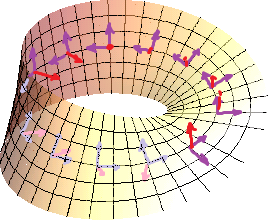
\includegraphics[width=0.2\linewidth]{pics/mobius-fibre.png}
    \caption{M\"obius Strip, 
        Credit:
        \href{https://www.quora.com/What-is-a-Fiber-Bundle-in-laymans-terms-What-is-it-used-for}{Quora} }
\end{figure}

\begin{thm}
    The set of Bloch functions (i.e. projectors) defines a map from the
    base space to $U(N_+ +N_-)/U(N_+)\times U(N_-)$. Topological
    distinct maps of this type can be classified by their homotopy
    group
    \begin{equation}
        \pi_{d+D}[U(N_+ +N_-)/U(N_+)\times U(N_-)]
    \end{equation}
\end{thm}

When $N_\pm$ is large enough, and when $d+D$ is even, this group is
$\mathbb{Z}$, the integer topological invariant is the Chern number.

\subsection{Winding number}
\label{sec:Winding-number}
\begin{itemize}
    \item Can only be defined in the presence of chiral symmetry.
    \item Relavant space: $U(N), \Rightarrow$
    \item $Q$ matrix (projector) Can be classified by
        $\pi_{d+D}[U(N)]$, which is nontrivial when $d+D$ is odd. When
        $d+D$ is odd, $\pi_{d+D}[U(N)]=\mathbb{Z}$, with maps
        characterized by the winding number.
\end{itemize}

\subsection{Chern-Simons invariant}
\label{sec:Chern-Simons-invariant}
\begin{itemize}
    \item Can be defined when $d+D$ is odd.
    \item Symmetry $\rightarrow$ Quantized/Discrete CS invariant. e.g.
        \begin{itemize}
            \item chiral symmetry quantizes CS
        \end{itemize}
    \item Not gauge-invariant.
        \begin{itemize}
            \item But $W:= \exp{2\pi i \,\text{CS}}$ is gauge-invariant.
        \end{itemize}
\end{itemize}

\subsection{Fu-Kane Invariant}
\label{sec:Fu-Kane-Invariant}
\begin{itemize}
    \item Construction requires special attention in the choice of basis
\end{itemize}

\subsection{K-theory Approach}
\label{sec:K-theory-Approach}
\begin{itemize}
    \item Topological nontrivial phases $\Rightarrow$ have massive
        Dirac Hamiltonian representatives
\end{itemize}
\section{Anchor}
\label{sec:Anchor}

\begin{thebibliography}{1}
    \bibitem{review}
    \url{http://journals.aps.org/rmp/abstract/10.1103/RevModPhys.88.035005}
\end{thebibliography}
\printnomenclature
\section{License}
The entire content of this work (including the source code
for TeX files and the generated PDF documents) by 
Hongxiang Chen (nicknamed we.taper, or just Taper) is
licensed under a 
\href{http://creativecommons.org/licenses/by-nc-sa/4.0/}{Creative 
Commons Attribution-NonCommercial-ShareAlike 4.0 International 
License}. Permissions beyond the scope of this 
license may be available at \url{mailto:we.taper[at]gmail[dot]com}.
\end{document}
